\documentclass[12pt]{report}
\usepackage{graphicx}                                   %% This package adds graphic options
\usepackage{subcaption}                                 %% This package modifies caption layout
\usepackage{threeparttable}                             %% This package modifies figure spacing
\usepackage{wrapfig}                                    %% This package allows text wrapping around figures
\usepackage{tikz}                                       %% This figure allows the IHG logo on title page
\usepackage{booktabs}                                   %% This package is for tables
\usepackage[export]{adjustbox}                          %% This package aligns photos within a table
\usepackage{array}                                      %% This package allows for customizing tables
\usepackage{rotating}                                   %% This package is for rotating tables
\usepackage{colortbl}                                   %% This package adds color to tables
\usepackage{fancyhdr}                                   %% This package adds fancy headers
\usepackage{multirow}                                   %% This package adds combined rows to tables
\usepackage{xcolor}                                     %% This package adds colors to the document
\usepackage{sectsty}                                    %% This package modifies chapters and sections
\usepackage[titles]{tocloft}                            %% This package modifies TOC layout
\usepackage[a4paper,margin=2.5cm,bottom=2cm]{geometry}  %% This package describes page layout
\usepackage{setspace}                                   %% This package is for line spacing
\usepackage{titlesec}                                   %% This package modifies section titles
\usepackage{enumerate}                                  %% This package is for numbered lists
\usepackage{siunitx}                                    %% This package is for SI unit abreviations
\usepackage[version=4]{mhchem}                          %% This package is for typing chemical components
\usepackage[backend=biber,style=apa,sortcites=yes]{biblatex}    %% This package is for refernces, APA, Sorting


\DeclareFieldFormat[article]{journaltitle}{#1}          %% Removes italics from bibliography
\DeclareFieldFormat[article]{volume}{#1}                %% Removes italics from bibliography
\DeclareFieldFormat[inbook]{booktitle}{#1}              %% Removes italics from bibliography
\DeclareFieldFormat[manual]{title}{#1}                  %% Removes italics from bibliography
\DeclareFieldFormat[report]{title}{#1}                  %% Removes italics from bibliography

\DeclareLanguageMapping{english}{english-apa}           %% Set the cites to APA english style
\addbibresource{sections/references.bib}                %% Add the bibilograph document

%% -------------------------------BELOW this for full citations hyperlinks--------------------------%%
%% -------------------------------BELOW this for full citations hyperlinks--------------------------%%
\DeclareCiteCommand{\cite}
  {\usebibmacro{prenote}}
  {\usebibmacro{citeindex}%
   \printtext[bibhyperref]{\usebibmacro{cite}}}
  {\multicitedelim}
  {\usebibmacro{postnote}}

\DeclareCiteCommand*{\cite}
  {\usebibmacro{prenote}}
  {\usebibmacro{citeindex}%
   \printtext[bibhyperref]{\usebibmacro{citeyear}}}
  {\multicitedelim}
  {\usebibmacro{postnote}}

\DeclareCiteCommand{\parencite}[\mkbibparens]
  {\usebibmacro{prenote}}
  {\usebibmacro{citeindex}%
    \printtext[bibhyperref]{\usebibmacro{cite}}}
  {\multicitedelim}
  {\usebibmacro{postnote}}

\DeclareCiteCommand*{\parencite}[\mkbibparens]
  {\usebibmacro{prenote}}
  {\usebibmacro{citeindex}%
    \printtext[bibhyperref]{\usebibmacro{citeyear}}}
  {\multicitedelim}
  {\usebibmacro{postnote}}

\DeclareCiteCommand{\parenciteA}[\mkbibparens]
  {\usebibmacro{prenote}}
  {\usebibmacro{citeindex}%
    \printtext[bibhyperref]{\printnames{labelname}, \printdate}}
  {\multicitedelim}
  {\usebibmacro{postnote}}

\DeclareCiteCommand{\footcite}[\mkbibfootnote]
  {\usebibmacro{prenote}}
  {\usebibmacro{citeindex}%
  \printtext[bibhyperref]{ \usebibmacro{cite}}}
  {\multicitedelim}
  {\usebibmacro{postnote}}

\DeclareCiteCommand{\footcitetext}[\mkbibfootnotetext]
  {\usebibmacro{prenote}}
  {\usebibmacro{citeindex}%
   \printtext[bibhyperref]{\usebibmacro{cite}}}
  {\multicitedelim}
  {\usebibmacro{postnote}}

\DeclareCiteCommand{\textcite}
  {\boolfalse{cbx:parens}}
  {\usebibmacro{citeindex}%
   \printtext[bibhyperref]{\usebibmacro{textcite}}}
  {\ifbool{cbx:parens}
     {\bibcloseparen\global\boolfalse{cbx:parens}}
     {}%
   \multicitedelim}
  {\usebibmacro{textcite:postnote}}


\DeclareCiteCommand{\citeauthor}
    {}
    {\bibhyperref{\printnames{labelname}}}
    {\multicitedelim}
    {}

\DeclareCiteCommand{\citeauthoryear}
    {}
    {\bibhyperref{\printnames{labelname} \printdate}}
    {\multicitedelim}
    {}

\DeclareCiteCommand{\citeauthoryearpar}
    {}
    {\bibhyperref{\printnames{labelname} \mkbibparens{\printdate}}}
    {\multicitedelim}
    {}

\DeclareCiteCommand{\citeyearpar}
    {}
    {\mkbibparens{\bibhyperref{\printdate}}}
    {\multicitedelim}
    {}

%% -------------------------------ABOVE this for full citations--------------------------%%
%% -------------------------------ABOVE this for full citations--------------------------%%


\usepackage{hyperref}                           %% Package is for hyperlinking refrences
\usepackage[nameinlink,capitalize]{cleveref}    %% Package for refrences,links entire name, capitalized "Fig."




%%===============================================PAGE SETUP==========================================================
  \hypersetup{                                %% Sets hyperlink style,
    colorlinks  =   true,                       %% All links are colored
    urlcolor    =   blue,                       %% DOI color is blue
    linkcolor   =   blue,                       %% Set link color
    linktoc     =   page,                       %% Only the TOC page numbers are linked "all"=page and title
    citecolor   =   blue}                       %% Set cite color

  \captionsetup{                              %% Sets format of figure and table captions
    labelsep        = period,                   %% Period label seperator
    skip            = 3pt,                      %% Sets the gap space between the figure and caption
    font            = {small,sf},               %% Small text, sans serif font
    labelfont       = bf,                       %% Fig and Table are bolded
    width			= .8\textwidth,			%% Sets the width of the captions
    singlelinecheck = false}                    %% Single line check

  \captionsetup[sub]{                         %% Sets format of figure and table  SUBcaptions
    font            = {footnotesize,sf},        %% Smaller text, sans serif font
%    labelfont       = normalfont,              %% Subcaption labels are normal font
    singlelinecheck = false}                    %% Single line check


\pagestyle{fancy}                           %% Sets up the headers and footers
    \fancyhead{}                                    %% clear all header fields
    \lhead{                                         %% Format the left header
      \fontsize{10}{12}\selectfont                  %% Font size
      \textcolor{gray}                                                  %% Text color
      {\bfseries Benthic Invertebrate Sampling and Monitoring}}         %% Bold font

%% Section title spacing
    \titlespacing*{\section}{0pt}{\baselineskip}{0\baselineskip}        %% No indent, 1 line above, 0 lines below
    \titlespacing*{\subsection}{0pt}{0\baselineskip}{0\baselineskip}    %% No indent, 0 lines above, 0 lines below
    \titlespacing*{\subsubsection}{0pt}{0\baselineskip}{0\baselineskip} %% No indent, 0 lines above, 0 lines below
    \makeatletter
    \renewcommand\paragraph{											%% Paragrah heading starts a new line
    	\@startsection{paragraph}{4}{0mm}%
    	{.25\baselineskip}
    	{.05\baselineskip}
    	{\normalfont\normalsize\bfseries}}
    \makeatother

%% Table set up
    \newcolumntype{B}[1]{>{\centering\arraybackslash}b{#1}}    %% Table paragraph collumn that is centered on the bottom
    \newcolumntype{R}[1]{>{\raggedleft\arraybackslash}b{#1}}   %% Table paragraph collumn that is right aligned on the bottom


%%================================================END PAGE SETUP============================================




%%=============================================BEGIN DOCUMENT===============================================

\begin{document}                            %% Begin the report document

    \onehalfspacing                                               %% Sets 1.5 line spacing

    \setlength{\parskip}{.4\baselineskip}%                        %% Sets the spacing between paragraphs
    \setlength{\parindent}{0pt}%                                  %% Removes the indents from paragaphs
    \renewcommand{\thesection}{\arabic{section}}                  %% Removes chapter number from headings

%%-----------------TITLE PAGE
  \begin{titlepage}

\begin{tikzpicture}[remember picture,overlay]                             %% Insert BOKU logo in upper right, .75cm margin
   \node[anchor=north east,inner sep=.75cm] at (current page.north east)
              {
\includegraphics[width=0.3\linewidth]{images/IHG}};         %% Color photo
\end{tikzpicture}

\begin{center}                                          %% Begin centering all the text
    \vspace*{3cm}                                           %% Insert vertical space

%%----------TITLE
    \LARGE                                                  %% LARGE text for the title
    \textbf{"Report Title"}

%%----------SUBTITLE
    \vspace{0.5cm}                                          %% Insert vertical space
    %Thesis Subtitle

    \vspace{1.5cm}                                          %% Insert vertical space

%%----------AUTHORS
    \Large                                                  %% Large text for the authos, class and date
    Jay Morgan - 11729236\\
    Max Loimer\\
    Andy Cosma\\
    Tonia Sosa\\
    \vspace{3cm}                                            %% Insert vertical space

%%----------CLASS
	812355 Fish sampling and monitoring\\
    812356 Fish ecological status assessment
    \vspace{.5cm}                                           %% Insert vertical space

%%----------DATE
    \today                                                  %% Insert today's date
    \vfill                                                  %% Fill the rest of the verticle space

    \end{center}                                            %% End centering of the text

%%----------INSTITUTE
    \normalsize                                             %% Normalesize text for the BOKU info
    Institute of Hydrobiology and Aquatic Ecosystem Management\\
    Department of Water, Atmosphere and Envrionment\\
    BOKU - University of Natural Resources and Life Sciences, Vienna\\





\end{titlepage}

                            %% Clears page and adds title page then clears page


%%-----------------ABSTRACT
    \onehalfspacing                                         %% Sets 1.5 line spacing
    \pagenumbering{roman}                                   %% Sets page number to roman numeral
    \fancyfoot{}                                            %% clear all footer fields (Hide page numbers)

  
\setcounter{secnumdepth}{0}                    %% Removes section number

\section{Abstract}
Most European rivers are impacted by various anthropogenic pressures and in need for action in order to reach a good ecological status as required by the EU Water Framework Directive. Since benthic invertebrates are good bio-indicators, they are often used to monitor rivers and to assess organic pollution, habitat availability and overall degradation. For this study the multi-habitat sampling approach was carried out in the unimpacted river Ois and in the channelized

\paragraph{thing}
 Maiergraben in order to assess differences in benthic invertebrate communities. At the unimpacted river different mineral habitats, biotic cover and flow velocities are present, whereas the impacted site is very homogenous. Furthermore, a higher number of taxa, EPT-Taxa and sensitive taxa occur at the Ois, which is a result of high habitat heterogeneity. The Maiergraben on the other hand shows low taxa diversity and very high abundances of generalists such as chironomids. In order to reach a good ecological status at the Maiergraben the need for action should not be ignored but appropriate measures should be implemented to restore the rivers biodiversity.




I added this to the abstrcat
                              %% Clears page and adds abstract page then clears page


%%----------------TABLE OF CONTENTS
    \onehalfspacing                                               %% Sets 1.5 line spacing
    \phantomsection                                                 %% Phantom section so TOC links here
    \setcounter{tocdepth}{4}                                        %% Inlcude sub-subsections in TOC
  \let\chapter\section\tableofcontents                            %% Insert TOC as a section
      \renewcommand{\cftsecfont}{\fontseries{b}\selectfont}         %% Set TOC sections to bold
      \addcontentsline{toc}{section}{Table of contents}             %% Add TOC to table of contents page


%%----------BODY
    \cleardoublepage                                        %% Reset page numbering
    \pagenumbering{arabic}                                  %% Page number in arabic
    \cfoot{\thepage}                                        %% Adds page numbers to footer

    \onehalfspacing                                         %% Sets 1.5 line spacing
    \setcounter{secnumdepth}{3}                             %% Adds sub-subsection number
%  

\section{Introduction}\label{sec:introduction}                                                   %% The first section

Limited access to clean water has become an increasingly alarming concern around the world. This is not the current situation in Austria, where most of the rivers have low levels of organic pollution. However, through the pursuit of hydropower production and flood protection, Austria’s water bodies face other anthropogenic pressures such as channelization, impoundment and hydropeaking~\parenciteA{Muhar2000}. The EU Water Framework Directive 2000/60/EC (WFD) established the legal obligation of member countries to maintain healthy water resources and mitigate damages inflicted upon their water bodies. The WFD describes a water body’s status by both abiotic and biotic criteria. Biological quality elements are subdivided into assessment of benthic invertebrates, fish, algae and aquatic flora. The ecological status of a water body is defined by comparing the biological community composition present with the near-natural reference conditions. The ecological status is calculated from the residual between the observed condition and the reference condition~\parenciteA{Furhacker2008}.

Benthic invertebrate organisms live in a diverse range of habitats representing a wide variety of aquatic ecosystems. Community structure of Macrozoobenthos (MZB) responds to environmental disturbances in a rather predictable way. This makes them an excellent candidate for monitoring changes in environmental conditions~\parenciteA{Li2010}. MZBs are able to reflect different anthropogenic pressures through changes in structure or function of the assemblages. These changes allow for an overall assessment of streams. Aside from organic pollution, MZB can detect habitat loss and overall stream degradation~\parenciteA{Hering2004, Hering2006}. According to~\textcite{Marzin2012}, macroinvertebrate metrics appear to be more sensitive to the degradation of the overall condition of the river than fish metrics. This could be explained by the localized nature of MZB. The insect order trichoptera are particularly well suited as a bioindicators for describing habitat degradation~\parenciteA{Schmidt-Kloiber2017}.

Many benthic invertebrate species have adapted to specific habitat parameters by way of flow velocity preference, structural needs, feeding strategies and tolerance to pollution~\parenciteA{Stoll2016}. It has been shown that substrate size is one of the best predictors of benthic invertebrate distribution within a river by~\textcite{Jowett2003} and~\textcite{Schroder2013}; while~\textcite{Dohet2015} described the influence that thermal regime and land use has on MZB inhabiting headwater streams. A study of species diversity and functional feeding groups of benthic invertebrates in Austrian rivers, which was carried out by~\citeauthoryearpar{Yoshimura2006}, showed that MZB communities are dependent on their environmental conditions. Studies in Poland have shown that benthic communities have significantly reduced taxonomic richness in constrained channels~\parenciteA{Wyzga2014}.

\begin{figure}[!htb]                                                       %% Reference site photo
  \center
  \includegraphics[width=.95\linewidth]{images/site_reference}                 %% Width, Image file COLOR
  \caption{Reference sample location on Ois River.}                            %% Figure Caption
  \label{fig:site_reference}                                                        %% Figure label key
\end{figure}


This report focuses on the benthic invertebrate communities sampled from two Alpine rivers near Lunz-am-see. We collected and assessed a sample of the benthic community from a near-natural site of the Ois River~(\cref{fig:site_reference}). This was to be used as a reference site when compared to a sample which was collected from a heavily impacted site of the Maiergraben. By comparing the collected samples from the Ois and Maiergraben, we aim to answer the following questions:

\singlespacing                                              %% Set single spacing
\begin{enumerate}
  \item Does habitat availability differ between the unimpacted Ois River and the impacted Maiergraben?
  \item Is there a relation between choriotope and sensitive screening taxa?
  \item What influence do microhabitats have on benthic communities within a river?
  \item Is there a difference in taxa composition, diversity and abundance between the unimpacted Ois and impacted Maiergraben?
  \item Does the benthic community represent the observed impacts at the Maiergraben?
\end{enumerate}
\onehalfspacing                                             %% Sets 1.5 line spacing


We hypothesized that the hydro-morphologically dynamic Ois River will contain more diverse habitat than the constrained Maiergraben. We predicted that some screening taxon are associated with specific choriotopes. We also hypothesized that habitat heterogeneity will result in more taxon richness and abundance, with an increase in specialized taxa. We predicted that the taxa composition, diversity and abundance would differ between the two sites, with the Ois River having a higher diversity and abundance than the Maiergraben. We assumed that the benthic community of the Maiergraben will be comprised of taxon associated with heavily impacted and channelized rivers.

                                   %% Adds introduction to report
%  

\section{Materials and Methods}\label{sec:material_methods}          %% The first section

\subsection{Study area}\label{sec:study_area}                %% The Study areas




The benthic macro-invertebrate samples were taken at two sites near lake Lunz (Mostviertel, lower Ausrtria). For reference conditions the Ois River in Lunz am See was sampled~(\cref{fig:site_reference}). This small, natural, alpine river represents the headwaters of the Ybbs River and subsequently flows into the Danube river. The second sampling site was the so called Maiergraben, a small, concreted, channelized creek flowing through a forested area into lake Lunz~(\cref{fig:site_impactedA}).



\begin{figure}[!htb]                                                        %% Impacted site photo
\centering                                                                  %% Center the figures
\subcaptionbox{Heavy regulation present at impacted site.\label{fig:site_impactedA}}{   %% First subcaption
  \includegraphics[width=0.48\columnwidth]{images/site_impacted1}}    %% Set width and select first image COLOR
  \hfill                                                                                    %% Fill Blank space
\subcaptionbox{Sample collection from impacted area.\label{fig:site_impactedB}}{        %% Second subcaption
  \includegraphics[width=0.48\columnwidth]{images/site_impacted2}}        %% Set width and second image COLOR
  \hspace*{\fill}                                                                           %% Fill blank space
\caption{Impacted site located on Maiergraben.}\label{fig:site_impacted}          %% Capition for both figures
\end{figure}




\subsection{Methods}\label{sec:methods}                         %% The methods section

\subsubsection{Multi-Habitat Sampling (MHS)}\label{sec:mhs}         %% Describe MHS


For this approach the examined river reach was partitioned into 20 subunits. These sampling units were representing different habitat types (choriotopes) and their proportional areal coverage within the reach. Sampling units were characterized by both mineral~(\cref{tab:choriotope_mineral}) and biotic~(\cref{tab:choriotope_biotic}) habitats.


\begin{table}[!htb]                                 %% Mineral choriotope table
  \small                                                       %%makes the table font small
  \centering
  \caption{Mineral choriotopes.}
    \begin{tabular}{ l l p{7cm} }
  \toprule
    Nomenclature  &
    \multicolumn{1}{c}{Grain size}  &
    \multicolumn{1}{c}{Description of choriotope} \\
  \hline
  \hline
    megalithal      & \textgreater 40 cm               & upper sides of boulders, large cobbles and blocks, bedrock\\
    macrolithal     & \textgreater 20 cm to 40 cm      & coarse blocks, head-sized cobbles, variable percentages of cobbles, gravel and sand\\
    mesolithal      & \textgreater 6.3 cm to 20 cm     & fist to hand-sized cobbles and pebbles with a variable percentage of gravel and sand\\
    microlithal     & \textgreater 2 cm to 6.3 cm      & pebbles, coarse gravel with percentages of medium to fine gravel\\
    akal            & \textgreater 0.2 cm to 2 cm      & fine to medium-sized gravel\\
    psammal         & 0.063 mm to 2 mm      & sand\\
    pelal           & \textless 0.063 mm            & mud and sludge\\
    argillal        &                       & silt, loam and clay\\
  \bottomrule
    \end{tabular}
  \label{tab:choriotope_mineral}%
\end{table}%


First the share of mineral habitat classes was defined, secondly the biotic habitats within the mineral habitats were classified. This was done by a visual estimation of the area. For every 5\% of a certain choriotope (combination of mineral and biotic habitat) one sampling unit was chosen. The shares and subunits of each choriotope were then put in a field-protocol~(see~\hyperref[appendixA]{Appendix A}).

Sampling units also had to be distributed accordingly between the mesohabitats (river bottom/bank, lentic/lotic, riffles/pools). As the sampling area should not be disturbed beforehand, the sampling started downstream and then proceeded upstream.


%\paragraph{Habitat Composition}\label{sec:choriotopes}         %% Describe chiriotopes



\begin{table}[!htb]                                 %% Biotic choriotope table
  \centering
  \small                                                       %%makes the table font small
  \caption{Biotic choriotopes.}
    \begin{tabular}{ l l }
  \toprule
    Nomenclature  &
    \multicolumn{1}{c}{Description of choriotope} \\
  \hline
  \hline
    algal periphyton    & areal stone cover\\
    filamentous algae   & tufts or floating mats\\
    mosses              & -\\
    macrophytes         & submerged plants\\
    living wood         & roots, branches (with leaves),\newline tree trunks\\
    deadwood            & branches and tree trunks\\
    CPOM                & course particulate matter\\
    FPOM                & fine particulate organic matter\\
    sapropel            & decaying sludge\\
    bacteria \& fungi   & lawns and tufts\\
  \bottomrule
    \end{tabular}
  \label{tab:choriotope_biotic}%
\end{table}%










\subsubsection{Sampling Method}\label{sec:sampling_method}          %% Describe impacted site

\begin{table}[!htb]                                         %% Ois Choriotopw Table
  \small                                                       %%makes the table font small
%  \centering
  \caption{Choriotope description of the sampling units at the Ois River.}
  \resizebox{\textwidth}{!}{                                                          %% Resizes the table to the text
  \begin{tabular}{ r b{.12\textwidth} b{.15\textwidth} c r r r }
    \toprule
    \multicolumn{1}{R{.08\textwidth}}{Sample} &
    \multicolumn{1}{B{.13\textwidth}}{Mineral Habitat} &
    \multicolumn{1}{B{.17\textwidth}}{Biotic \par\noindent Habitat} &
    \multicolumn{1}{B{.15\textwidth}}{Velocity \par\noindent [m/s]} &
    \multicolumn{1}{B{.08\textwidth}}{Velocity Class} &
    \multicolumn{1}{B{.08\textwidth}}{Water Depth \par\noindent [cm]} &
    \multicolumn{1}{B{.1\textwidth}}{Distance \par\noindent to Shore\par\noindent [m]} \\
    \hline
    \hline
    1\_2 & mesolithal & micro\_algae & 0.9   & high  & 10    & 2 \\
    3\_4 & macrolithal & micro\_algae\_moss & 1.3   & very\_high & 25    & 6 \\
    5\_6 & megalithal & moss  & 1.3   & very\_high & 5     & 8 \\
    7\_8 & mesolithal & micro\_algae & 0.5   & medium & 20    & 4 \\
    9\_10 & megalithal & micro\_algae & 0.5   & medium & 10    & 8 \\
    11\_12 & mesolithal & periphyton & 0.2   & slow  & 30    & 5 \\
    13\_14 & akal & none  & 0.2   & slow  & 25    & 2 \\
    15\_16 & mesolithal & CPOM  & {  0}     & no\_flow & 20    & 0.5-1 \\
    17\_18 & macrolithal & micro\_algae & {  0}     & no\_flow & 10    & 0.5 \\
    19\_20 & mesolithal & CPOM  & 0.2   & slow  & 20    & 0.5 \\
    \bottomrule
    \end{tabular}}%
  \label{tab:choriotope_ois}%
\end{table}%



Sample collection at each sampling unit was performed with a stationary rectangular net (Mesh size: \SI{500}{\micro\meter} EU standard) and by disturbing a quadratic area upstream of the net (25x25cm). For the Ois River we chose 10 sampling locations where we took 2 samples each, for a total of 20 units~(\cref{tab:choriotope_ois}).




Since the Maiergraben had a very homogenous structure we chose only four sampling locations – three in the creek and one under a small bridge. We collected 5 samples from each location for a total of 20 sampling units.~(\cref{tab:choriotope_maiergraben,fig:site_impactedB})


\begin{table}[!htb]
  \small                                                       %%makes the table font small
  %\centering
  \caption{Choriotope description of the sampling units at the Maiergraben.}
  \resizebox{\textwidth}{!}{                                                          %% Resizes the table to the text
  \begin{tabular}{ r b{.12\textwidth} b{.18\textwidth} c r r r }
    \toprule
    \multicolumn{1}{R{.08\textwidth}}{Sample} &
    \multicolumn{1}{B{.13\textwidth}}{Mineral Habitat} &
    \multicolumn{1}{B{.17\textwidth}}{Biotic \par\noindent Habitat} &
    \multicolumn{1}{B{.15\textwidth}}{Velocity \par\noindent [m/s]} &
    \multicolumn{1}{B{.08\textwidth}}{Velocity Class} &
    \multicolumn{1}{B{.08\textwidth}}{Water Depth \par\noindent [cm]} &
    \multicolumn{1}{B{.1\textwidth}}{Distance \par\noindent to Shore\par\noindent [m]} \\
    \hline
    \hline
    1-5   & technomega & micro\_macro\_algae & 0.22-0.32 & medium & 4.8   & 0.5 \\
    6-10  & technomega & micro\_macro\_algae & 0.24-0.34 & medium & 2.8   & 0.5 \\
    11-15 & technomega & micro\_macro\_algae & 0.22-0.32 & medium & 4.5   & 0.5 \\
    16-20 & technomega & bare  & 0.30-0.40 & medium & 4.2   & 0.5 \\
    \bottomrule
    \end{tabular}}%
  \label{tab:choriotope_maiergraben}%
\end{table}%


Samples taken from organic habitats, always had to include the underlying mineral substrates. The different mineral habitats needed to be sampled accordingly.
\begin{list}{}
  \item {\textbf{Megalithal:} Boulders were sampled from all sides by sweeping the surface with a brush and flushing the animals into the net.}
  \item {\textbf{Macro- and Mesolithal:} Surface dwelling animals were flushed in the net by gently sweeping the cobbles or stones by hand. Next clingers and sessile animals were scratched off with a brush. Finally, the underlying substrate (within 15 to 20 cm depth) was churned by foot.}
  \item {\textbf{Microlithal and Akal:} Coarse gravel and sandy substrate was sampled by disturbing the sediment by kicking it downstream the net.}
\end{list}

After sampling each unit, the content of the net was transferred first into a tray and then into a closable bucket, which was filled with ethanol, in order to kill the animals.


\subsubsection{Sorting Techniques}\label{sec:sorting_technigues}      %% Describe impacted site

To sort the animals by size classes the buckets contents were later put through a sieve tower with different mesh sizes (\SI{10}{\milli\meter} down to \SI{500}{\micro\meter}). The different fractions were then placed in trays~(\cref{fig:sorting_tray}), so animals could be sorted, counted and determined to screening taxa level with the help of binoculars~(\cref{fig:sorting}). Only whole animals, so no single body parts, empty shells, exuvies or headless animals were taken into account. In trays with large amounts of animals (usually the smaller fractions) rare or single-occurring animals were taken out, and the rest was subsampled. This was done by transferring the animals in another tray that consisted of a grid, separating the tray into 16 or 8 cells. The organisms of usually two representing subsamples were determined and counted. The number of animals then had to be multiplied accordingly.
A taxa list was created with MS Excel and further analysis were made with the programs MS Excel and EcoProf (version 4.0.0).






\begin{figure}[!htb]                               %% Sample processing
\centering                                                                  %% Center the figures
\captionbox{Sorting tray used for taxa identification.\label{fig:sorting_tray}}{   %% First subcaption
  \includegraphics[height=7.6cm]{images/sorting_tray}}         %% Set width and select first image COLOR
  \hfill                                                                                    %% Fill Blank space
\captionbox{Identifying taxa within the samples using binoculars.\label{fig:sorting}}{     %% Second subcaption
  \includegraphics[height=7.6cm]{images/sorting}}        %% Set width and second image COLOR
  \hspace*{\fill}                                                                    %% Fill blank space
\end{figure}




\subsection{Equipment}\label{sec:equipment}                 %% The equipment section


\begin{table}[htbp]
  \centering
    \begin{tabular}{l b{3cm} l}
    ·         Nets & ·   &      Sieve tower \\
                &   &\\
    ·         Brushes & · &        Sorting trays~(\cref{fig:sorting_tray}) \\
                &   &\\
    ·         Trays & ·    &     Subsampling trays \\
                &   &\\
    ·         Buckets (closeable) & ·  &       Tweezers \\
                &   &\\
    ·         Ethanol & ·     &    Binoculars \\
    \end{tabular}%
  \label{tab:addlabel}%
\end{table}%


                                        %% Adds methods to report
  	\section{Results}

\subsection{Ois River}\label{sec:ois_river}       %% Ois river




\subsubsection{Length-frequency distribution}\label{sec:ois_fish_lf}

This distribution of salmonid length in the investigated area of the Ois ranged from 45mm to 433mm.
72\% of the total catch had a length of less than 120mm, which is the threshold for young-of-the-year (YOY) fish.
Distribution of adult fish can be see in~\cref{fig:avg_length}.
Fish length among the mesohabitats trends toward the largest fish in pools, decreasing in size to runs and then riffles containing the smallest fish.
The median length of brown trout was similar in the riffle and run sections.

The Rothschild section of the river had similar length brown trout populations when compared to the Hinterleiten.
The rainbow trout populations in the Rothschild were significantly larger than that of the Hinterleiten in all three mesohabitats.
Additionally, the rainbow trout populations in all sampled areas were larger than the brown trout populations.

\begin{figure}[!htb]                              %% Average length of 1+ years
	\center
	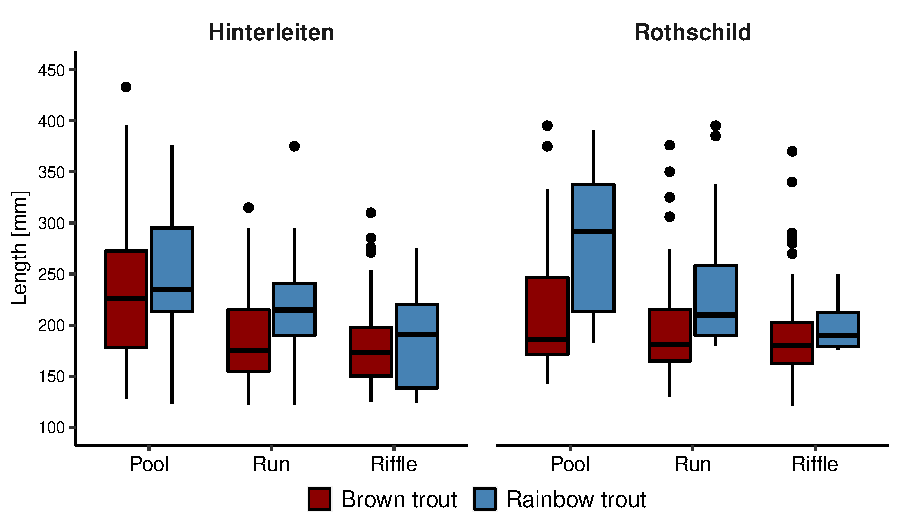
\includegraphics[width=.7\textwidth]{images/avg_length.pdf}                %% Width, Image file COLOR
	\caption{Boxplots displaying length of adult fish in investigated mesohabitats.}      %% Figure Caption
	\label{fig:avg_length}                                                       %% Figure label key
\end{figure}


\paragraph{Brown trout (\textit{Salmo trutta})}\label{sec:ois_bt_lf}

A very healthy brown trout population can be seen in the length-frequency chart of the combined sample areas~(\cref{fig:brown_single}).
A total of 1866 brown trout were caught in 9 sample sites.
Fish of less than 120mm in length represent the YOY, while the 1+ age class (\textgreater120mm) and 2+ age class (\textgreater220mm) are clearly visible along with several individuals larger than 300mm.
YOY fish account for the majority of the catch at 74\%, indicating successful spawning.

\begin{figure}[!htb]                              %% Brown in Ois
	\center
	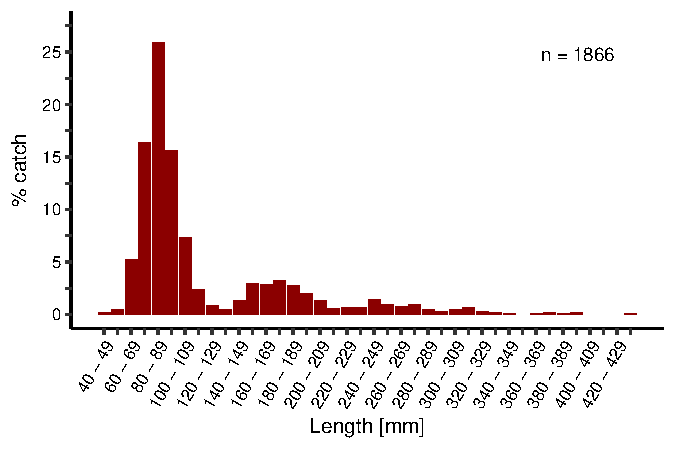
\includegraphics[width=.7\textwidth]{images/brown_single.pdf}                %% Width, Image file COLOR
	\caption{Length-frequency plot showing population structure of brown trout in the River Ois.}        %% Figure Caption
	\label{fig:brown_single}                                                       %% Figure label key
\end{figure}

Comparing the length-frequency of the two sampled sections~(\cref{fig:brown_section}) shows that the Hinterleiten has a higher portion of YOY at approximately 80\% of the total catch, while The 1+ fish accounted for only 13\% of total catch.
The YOY in the Rothschild section accounted for 60\% of total catch and the 1+ age class represented around 28\% of total catch.

\begin{figure}[!htb]                              %% Brown in section
	\center
	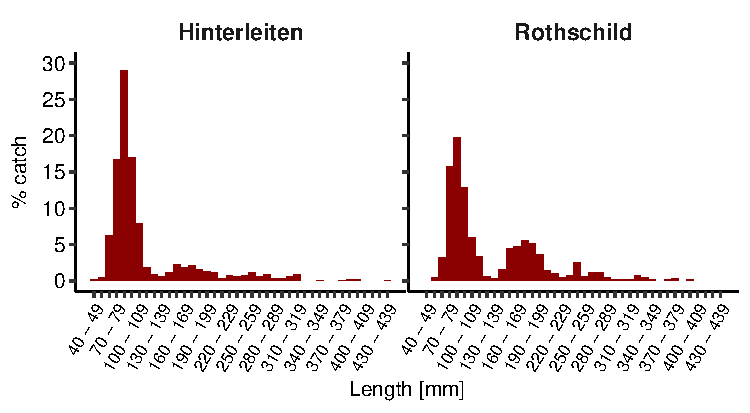
\includegraphics{images/brown_section.pdf}                %% Width, Image file COLOR
	\caption{Length-frequency plot showing the difference in population structure of brown trout in two sections of the River Ois.}   %% Figure Caption
	\label{fig:brown_section}                                                       %% Figure label key
\end{figure}

A comparison of brown trout populations in different mesohabitats can be seen in~\cref{fig:brown_meso}.
All age classes are present in the pool habitat, with YOY accounting for less than 50\% total catch.
1+ and 2+ fish accounted for 28\% and 15\% of the pools respectively.
Run mesohabitats contained more juvenile fish with YOY representing 72\% of the population.
21\% of the population were 1+ fish leaving less than 7\% fish greater than 220mm in length.
The riffles contained the highest percentage of YOY at 87\%.
1+ fish made up 11\% of the population, with very few fish larger than 220mm.

\begin{figure}[!htb]                              %% Brown in meso
	\center
	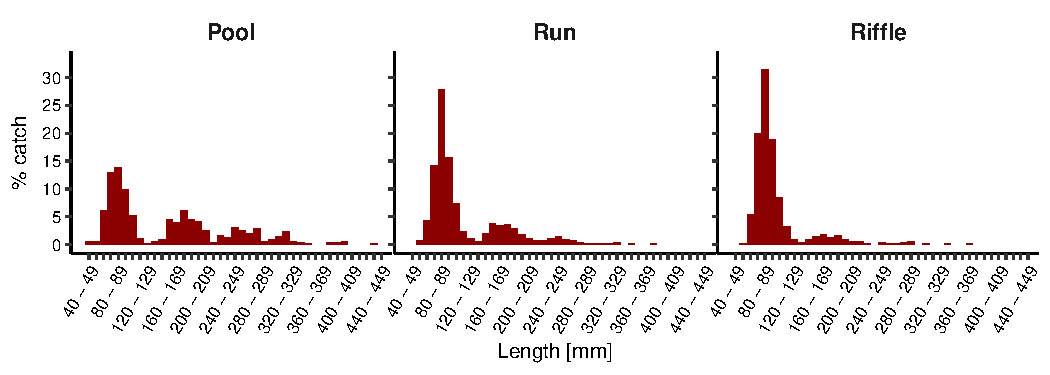
\includegraphics[width=\textwidth]{images/brown_meso}                %% Width, Image file COLOR
	\caption{Length-frequency plot of brown trout populations in different mesohabitats of River Ois.}        %% Figure Caption
	\label{fig:brown_meso}                                                       %% Figure label key
\end{figure}

A representation of the brown trout population in each of the sampled sites is shown in~\cref{fig:brown_mix}.
It can be seen that larger fish tend to occur most often in pool mesohabitats, less frequently in runs, and rarely in riffles.
YOY represent the majority of caught fish in the riffles and runs of all three sections.
The lower riffle of the Hinterleiten contained the youngest population with YOY accounting for 92\% of total catch.
All mesohabitats within the Rothschild showed a higher proportion of large fish when compared with the Hinterleiten habitats.
The Rothschild pool was unique in that YOY represented only 29\% of the catch, with 1+ fish (48\%), 2+ fish (17\%) and fish larger than 300mm (6\%) accounting for the remainder.

\begin{figure}[!htb]                              %% Brown mixed grid
	\center
	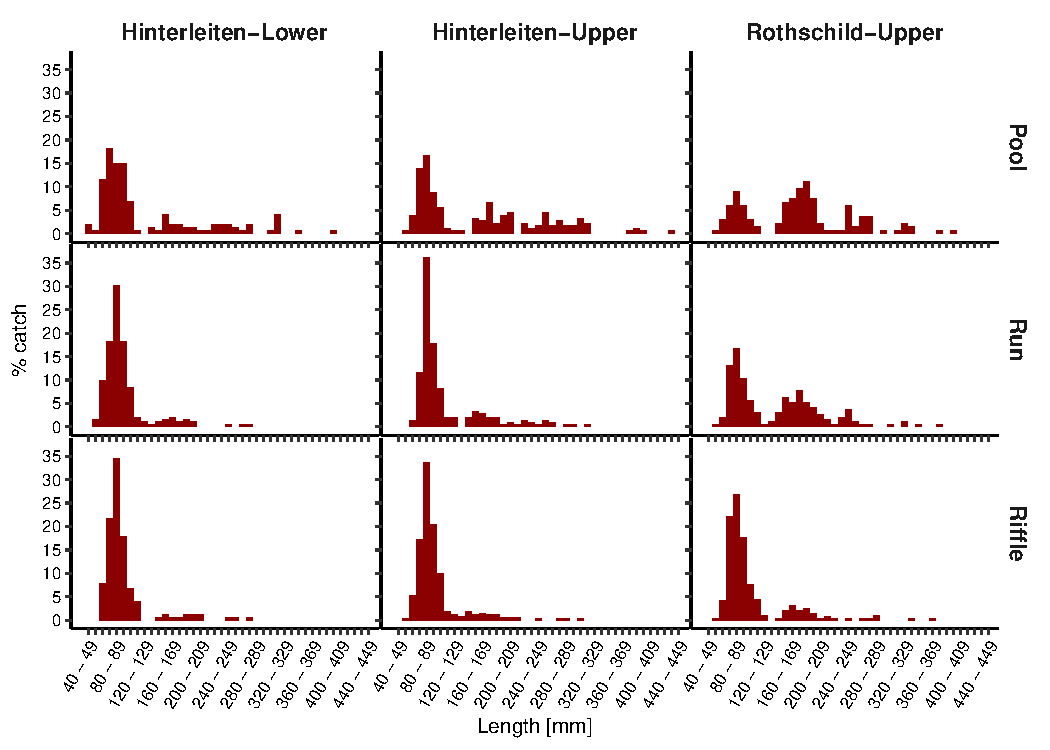
\includegraphics[width=\textwidth]{images/brown_mix}                %% Width, Image file COLOR
	\caption{Length-frequency plots of brown trout in the 9 sampled sections.}        %% Figure Caption
	\label{fig:brown_mix}                                                       %% Figure label key
\end{figure}


\paragraph{Rainbow trout (\textit{Onchorhynchus mykiss})}\label{sec:ois_rt_lf}

The population structure of rainbow trout sampled in the Ois can be seen in~\cref{fig:rain_single}.
All ages classes are present, with a high percentage of YOY fish.
Rainbow trout YOY were defined as individuals less than 150mm in length and accounted for 67\% of the 383 rainbow trout that were sampled.
1+ fish (\textgreater150mm) were 20\%, 2+ fish (\textgreater250mm) were 10\% and fish larger than 350mm were less than 3\% of the total catch.

\begin{figure}[!h]                              %% Rainbow in Ois
	\center
	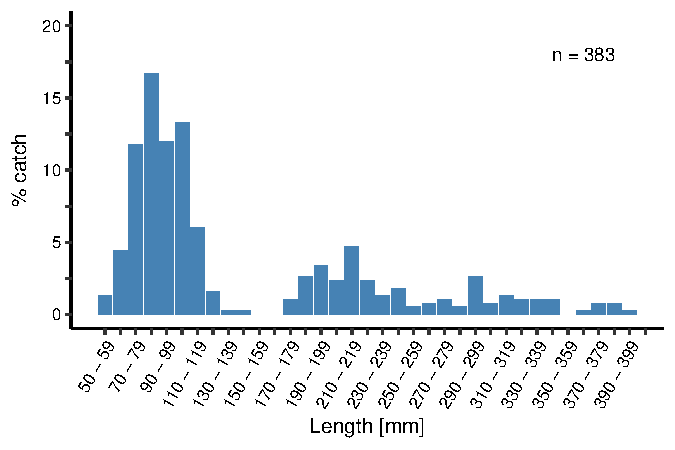
\includegraphics[width=.7\textwidth]{images/rain_single.pdf}     %% Width, Image file COLOR
	\caption{Length-frequency plot showing population structure of rainbow trout in the River Ois.}        %% Figure Caption
	\label{fig:rain_single}           %% Figure label key
\end{figure}

The rainbow trout populations between the two sections are quite similar~(\cref{fig:rain_section}) with the Rothschild having a slightly older population.
YOY had the highest portion of total catch in the Hinterleiten with 70\% and 63\% in the Rothschild.
1+ fish were comparable with 19\% and 20\%.
The share of 2+ fish was lower in the Hinterleiten (10\%) than the Rothschild (12.5\%).
350mm plus fish were mostly absent from the Hinterleiten, but contributed 6\% of the total catch in the Rothschild.

\begin{figure}[!h]                              %% Rainbow in sections
	\center
	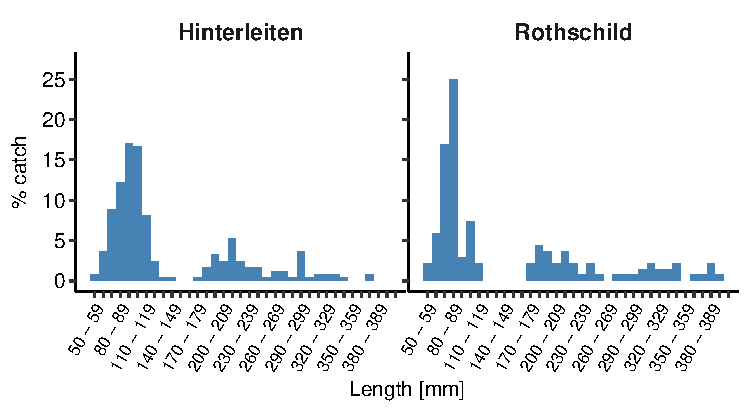
\includegraphics{images/rain_section.pdf}    %% Width, Image file COLOR
	\caption{Length-frequency plot showing the difference in population structure of rainbow trout in two sections of the River Ois.} %% Figure Caption 
	\label{fig:rain_section}     %% Figure label key
\end{figure}

The age class distribution of rainbow trout among the mesohabitats~(\cref{fig:rain_meso}) is comparable to the brown trout~(\cref{fig:brown_meso}).
The pool sections are characterized by an almost even distribution among the age classes.
The pools were composed of 38\% YOY, 31\% 1+ fish, 27\% 2+ fish and 4\% were larger than 350mm.
The runs had a younger population structure with 71\% of the total catch being YOY. 1+ fish (22\%), 2+ fish (5\%) and \textgreater350mm fish made up just over 2\% in the remainder of the runs.
Riffles had the youngest population by far, with 91\% being YOY.
The riffles also contained 7\% 1+ fish, 2\% 2+ fish and no fish larger than 350mm.

\begin{figure}[!htb]                              %% Rainbow in Meso
	\center
	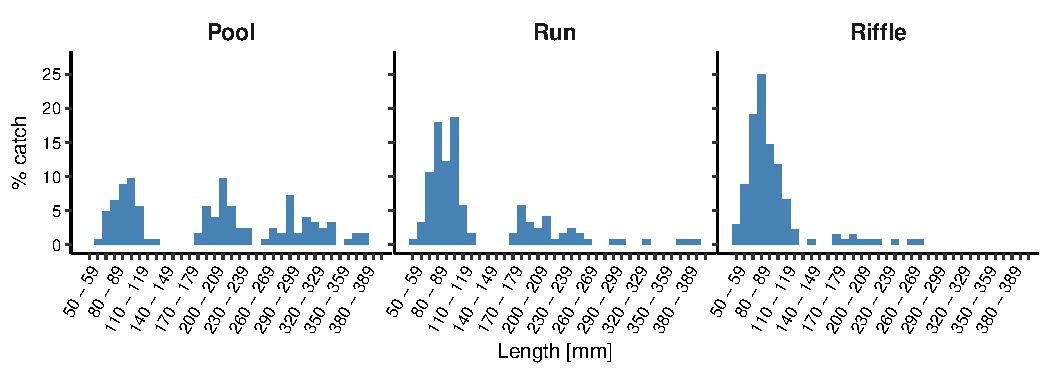
\includegraphics[width=\textwidth]{images/rain_meso.pdf}                %% Width, Image file COLOR
	\caption{Length-frequency plot of rainbow trout populations in different mesohabitats of River Ois.}        %% Figure Caption
	\label{fig:rain_meso}                                                       %% Figure label key
\end{figure}

The length-frequency of rainbow trout the sampled sections~(\cref{fig:rain_mix}) also follow the trends identifiable in the brown trout~(\cref{fig:brown_mix}).
Larger fish can be found in the pools, while more juveniles are found in runs and riffles.
Populations between the three sections are quite similar.
More detailed analysis is not possible due to the small sample size.

\begin{figure}[!htb]                              %% Rainbow in mixed grid
	\center
	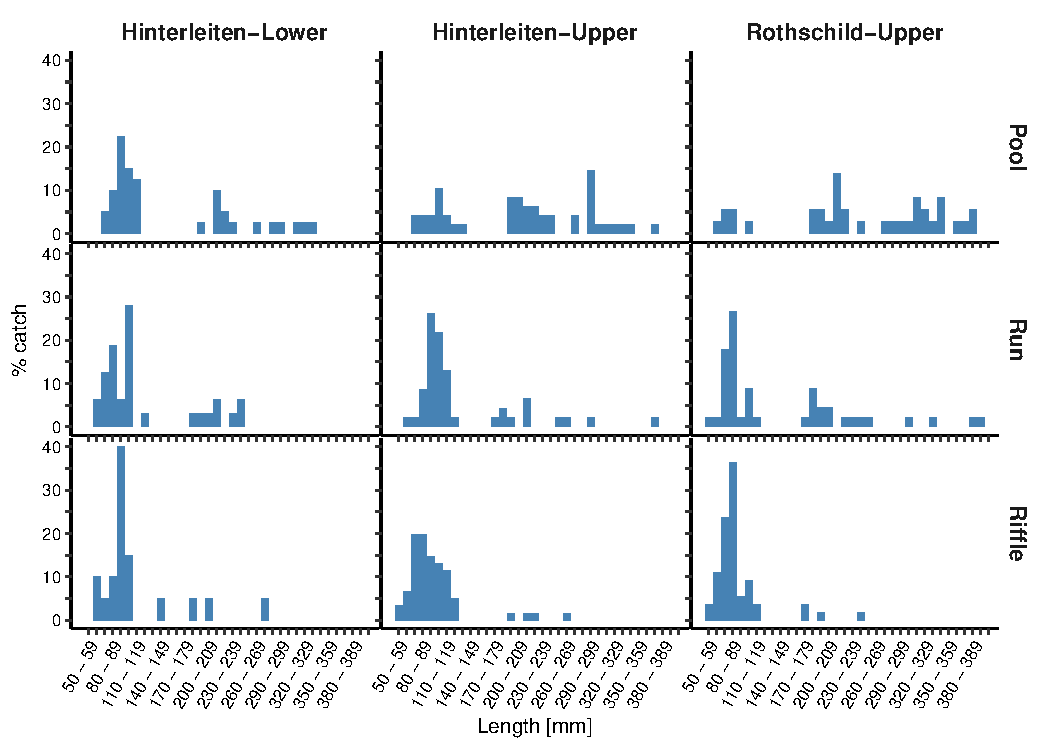
\includegraphics[width=\textwidth]{images/rain_mix.pdf}                %% Width, Image file COLOR
	\caption{Length-frequency plots of rainbow trout in the 9 sampled sections.}        %% Figure Caption
	\label{fig:rain_mix}                                                       %% Figure label key
\end{figure}


















\subsubsection{Abundance and Biomass}\label{sec:ois_ab_mass}

The sum of total catch for each sampled site was divided by the area sampling to calculate abundance and biomass.
These values were then weighted according to the habitat distribution of the Hinterleiten and Rothschild sections.
The ratio of mesohabitats can be seen in~\cref{tab:habitat_distribution}.

\begin{table}[!htb]                                 %% Habitat distribution
	\small                   
	\centering
	\caption{Habitat distribution among the river sections.}
	\begin{tabular}{ l c c }
		\toprule
		&	Hinterleiten  	&	Rothschild 	\\
		mesohabiat	&	\scriptsize[\%]	&	\scriptsize[\%]	\\
		\hline
		\hline
		pool	&	30	&	10	\\
		run     & 	27  & 	50	\\
		riffle  & 	43  & 	40	\\
		\bottomrule
	\end{tabular}
	\label{tab:habitat_distribution}%
\end{table}%

The combined abundance and biomass of all salmonid species can be seen in~\cref{fig:AB_all_species}.
The calculated abundance of the Hinterleiten was 2922 individuals per hectare.
Of those individuals, 1299 could be found in riffles, 1016 in pools, and 607 in runs.
The Rothschild had slightly less abundance at 2396 individuals per hectare.
Of these, 1065 could be found in riffles, 777 in runs, and 553 individuals in pools.
Due to habitat distribution, the Hinterleiten had a higher abundance than the Rothschild.


\begin{figure}[!htb]                              %% All species
	\center
	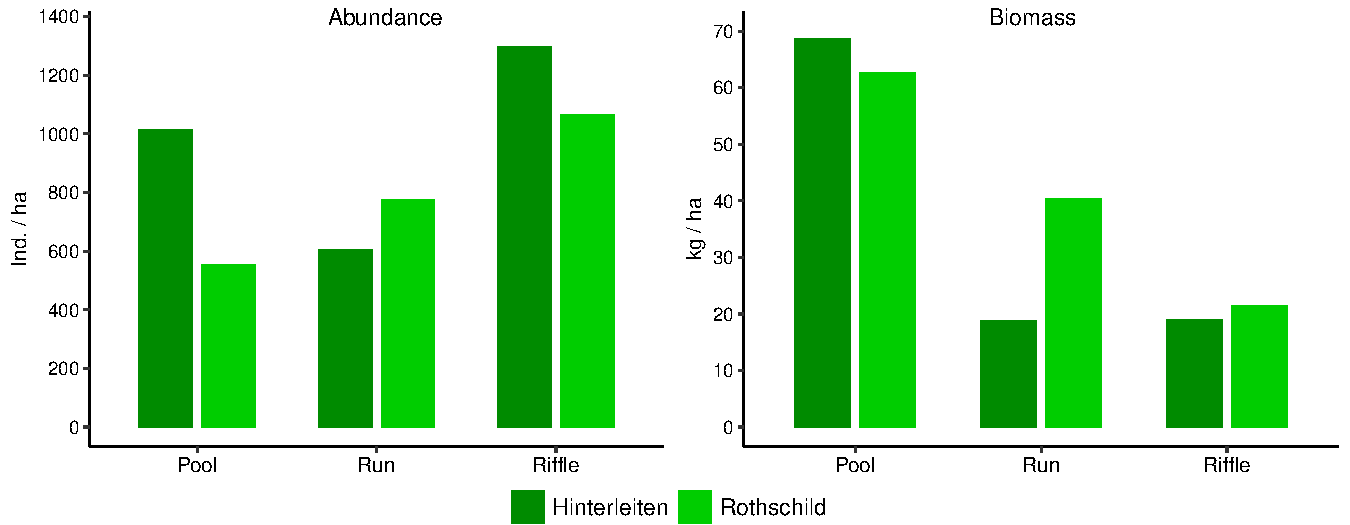
\includegraphics[width=.9\textwidth]{images/all_species.pdf}                %% Width, Image file COLOR
	\caption{Weighted distribution of combined abundance and biomass of salmonid species in the mesohabitats of two sampled sections.}        %% Figure Caption
	\label{fig:AB_all_species}                                                       %% Figure label key
\end{figure}

\begin{figure}[!htb]                              %% Brown trout
	\center
	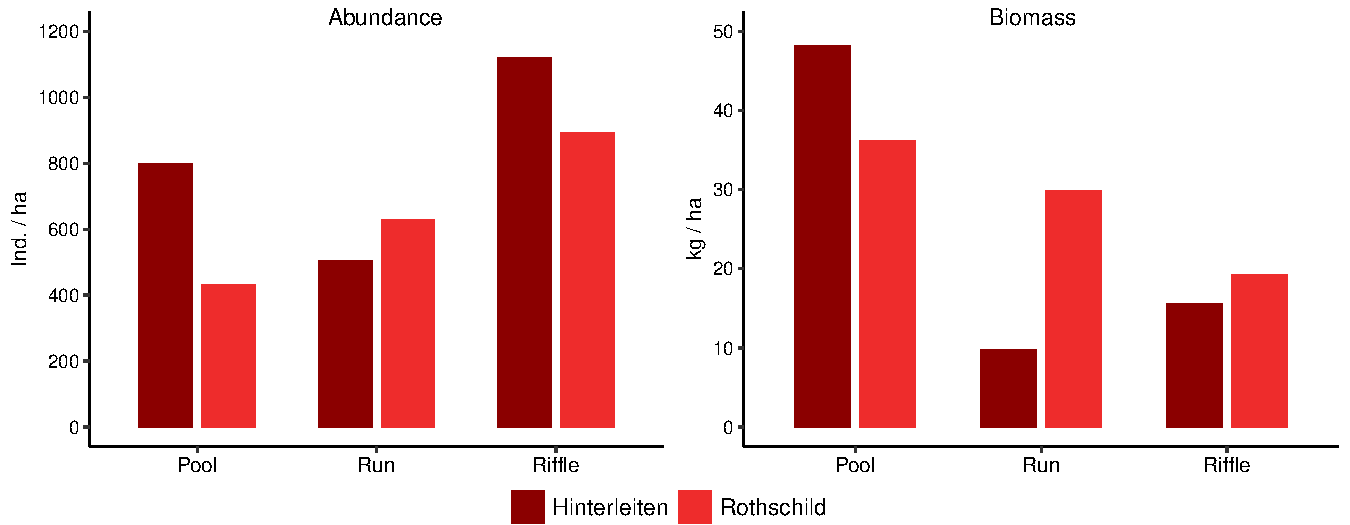
\includegraphics[width=.9\textwidth]{images/brown_trout.pdf}                %% Width, Image file COLOR
	\caption{Weighted distribution of abundance and biomass of brown trout population in the mesohabitats of two sampled sections.}        %% Figure Caption
	\label{fig:AB_brown}                                                       %% Figure label key
\end{figure}

\begin{figure}[!htb]                              %% Rainbow trout
	\center
	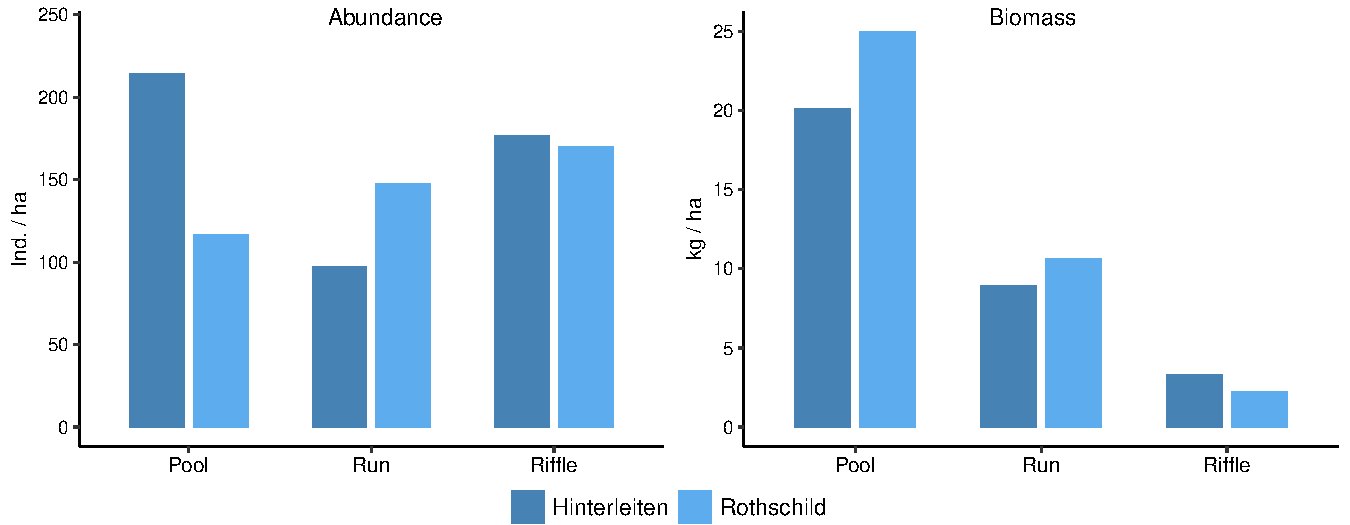
\includegraphics[width=.9\textwidth]{images/rainbow_trout.pdf}                %% Width, Image file COLOR
	\caption{Weighted distribution of abundance and biomass of rainbow trout population in the mesohabitats of two sampled sections.}        %% Figure Caption
	\label{fig:AB_rainbow}                                                       %% Figure label key
\end{figure}

%			\begin{figure}[!htb]                              %% Grayling
%				\center
%				\includegraphics[width=.9\textwidth]{images/grayling.pdf}                %% Width, Image file COLOR
%				\caption{Abundance and biomass of grayling in mesohabitats.}        %% Figure Caption
%				\label{fig:AB_gray}                                                       %% Figure label key
%			\end{figure}

\begin{figure}[!htb]                              %% All species in meso habitats
	\center
	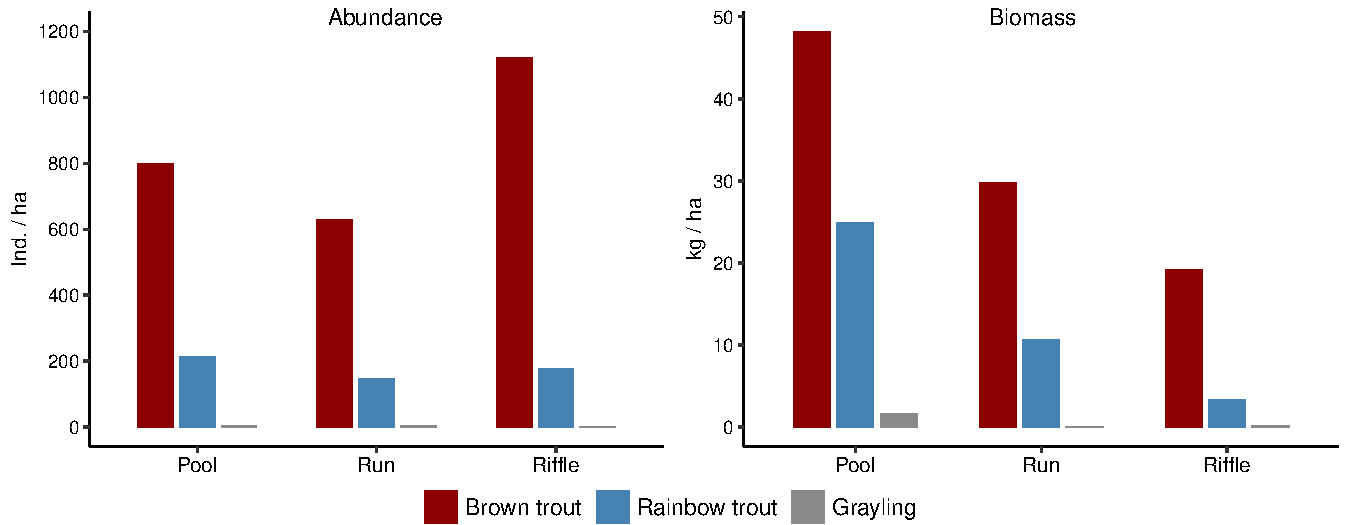
\includegraphics[width=.9\textwidth]{images/mesohabitat.pdf}                %% Width, Image file COLOR
	\caption{Comparison of the distributed abundance and biomass of salmonid species in mesohabitat components of the River Ois.}        %% Figure Caption
	\label{fig:AB_meso}                                                       %% Figure label key
\end{figure}

\begin{figure}[!htb]                              %% All species in sections
	\center
	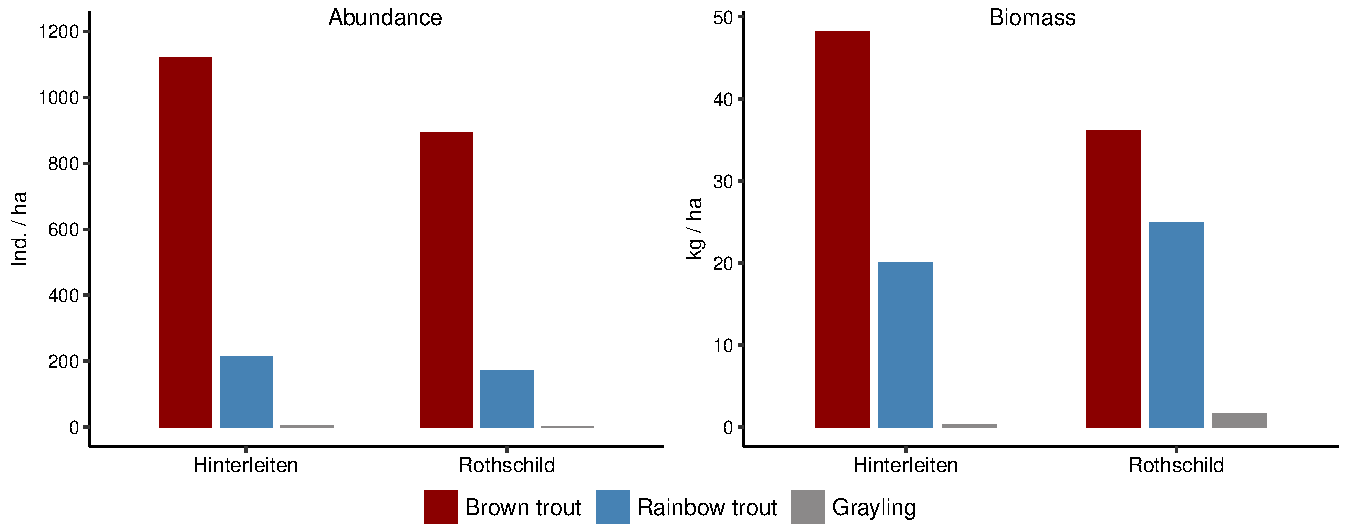
\includegraphics[width=.9\textwidth]{images/section.pdf}                %% Width, Image file COLOR
	\caption{Comparison of distributed abundance and biomass of salmonid species in Hinterleiten and Rothschild sections.}        %% Figure Caption
	\label{fig:AB_section}                                                       %% Figure label key
\end{figure}



\begin{table}[!htb]                                 %% Habitat distribution
	\small                   
	\centering
	\caption{Habitat distribution among the river sections.}
	\begin{tabular}{lllllllllll}
		\toprule
		 &  &  & Hinterleiten &  &  &  &  & Rothschild &  &  \\
		 & Habitat.dis & Ind.ha & kg.ha & Ind.ha.dis & kg.ha.dis & Habitat.dis & Ind.ha & kg.ha & Ind.ha.dis & kg.ha.dis \\
		 \hline
		 \hline
		All Species & \% &  &  &  &  & \% &  &  &  &  \\
		Pool & 30 & 3387 & 229.0 & 1016 & 68.7 & 13 & 4193 & 475.2 & 553 & 62.7 \\
		Run & 27 & 2247 & 69.5 & 607 & 18.8 & 47 & 1661 & 86.5 & 777 & 40.5 \\
		Riffle & 43 & 3022 & 44.3 & 1299 & 19.1 & 40 & 2644 & 53.3 & 1065 & 21.5 \\
		Brown trout &  &  &  &  &  &  &  &  &  &  \\
		Pool & 30 & 2661 & 160.8 & 798 & 48.3 & 13 & 3286 & 273.8 & 434 & 36.2 \\
		Run & 27 & 1874 & 36.2 & 506 & 9.8 & 47 & 1346 & 63.8 & 630 & 29.9 \\
		Riffle & 43 & 2606 & 36.2 & 1120 & 15.6 & 40 & 2213 & 47.7 & 892 & 19.2 \\
		Rainbow trout &  &  &  &  &  &  &  &  &  &  \\
		Pool & 30 & 714 & 67.0 & 214 & 20.1 & 13 & 883 & 189.2 & 117 & 25.0 \\
		Run & 27 & 360 & 33.2 & 97 & 9.0 & 47 & 315 & 22.7 & 148 & 10.6 \\
		Riffle & 43 & 411 & 7.8 & 177 & 3.3 & 40 & 423 & 5.6 & 170 & 2.3 \\
		Grayling &  &  &  &  &  &  &  &  &  &  \\
		Pool & 30 & 12 & 1.1 & 4 & 0.3 & 13 & 25 & 12.2 & 3 & 1.6 \\
		Run & 27 & 13 & 0.1 & 3 & 0.0 & 47 & 0 & 0.0 & 0 & 0.0 \\
		Riffle & 43 & 5 & 0.3 & 2 & 0.2 & 40 & 0 & 0.0 & 0 & 0.0 \\
		\bottomrule
	\end{tabular}
\end{table}

                                        %% Adds results to report
%    \section{Results}\label{sec:results}




\subsection{Screening Method}\label{sec:screening_method}       %% Screening Methond

A comparison of the river Ois and the Maiergraben was made using EcoProf~(\cref{fig:ecoprof}). Both rivers are located in the bioregion limestone prealps and the basic condition for general degradation is set to 1.5. More screening taxa in general and among them more sensitive taxa were found in the Ois than in the Maiergraben (see~\hyperref[appendixB]{Appendix B} for full taxon lists). Furthermore, the degradation-score is very high for the Ois, but the Maiergraben does not reach the expected value of 75. The saprobity-score is below 1 for the Ois and just above 1 for Maiergraben, which indicates that organic pollution is not a significant problem for either river. EcoProf showed that the Ois has very good status, while there is a need for action in the Maiergraben. This is due to general degradation as suggested by the low number of occurring sensitive taxa and the low degradation score.

\begin{figure}[!htb]                              %% EcoProf
  \center
  \includegraphics[width=.8\linewidth]{images/ecoprof}                %% Width, Image file COLOR
  \caption{EcoProf output for the Screening Method comparing the river Ois with Maiergraben.}        %% Figure Caption
  \label{fig:ecoprof}                                                       %% Figure label key
\end{figure}




\subsection{Microhabitats}\label{sec:microhabitats_results}       %% Microhabitats

The choriotope composition of the sites can be found in~\cref{fig:choriotope_composition} with more general habitat characteristics available in~\cref{tab:choriotope_ois,tab:choriotope_maiergraben}. From the first view it is obvious that in the Ois more diverse mineral habitats and biotic choriotopes are available. In the Ois the dominating mineral habitat is the mesolithal with a share of 50\% followed by macro- and megalithal with a share of 20\% each. Additionally, a small proportion with a share of 10\% of the river stretch is covered with sand. On the other hand, in the Maiergraben only technomegalithal is available for colonisation, making the river stretch very monotonous.


\begin{figure}[!htb]                               %% Choriotope composition
  \center
  \includegraphics[width=.9\linewidth]{images/choriotope_mineral}                 %% Width, Image file COLOR
  \includegraphics[width=.9\linewidth]{images/choriotope_biotic}                 %% Width, Image file COLOR
      \caption{Habitat Composition: The mineral choriotope composition of Ois (upper left) and Maiergraben (upper right) and the biotic choriotope composition of Ois (lower left) and Maiergraben (lower right).}      %% Figure Caption
  \label{fig:choriotope_composition}                                                        %% Figure label key
\end{figure}


The lower pie-charts in~\cref{fig:choriotope_composition} show the biotic choriotope composition of the rivers. In the Ois, the largest percentage of mineral habitats are covered by micro algae with a share of 40\% and CPOM with 20\%. The remaining river stretch is covered by equal parts of periphyton, moss or micro algae/moss. The Maiergraben shows less diverse biotic choriotopes and is dominated by micro/macro algae which cover 15 out of 20 sampling sites. The remaining five sampling sites lie bare.



\subsection{Taxa Composition}\label{sec:taxa_composition_results}       %% Taxa compsition

In the following section the taxa composition of the rivers Ois and Maiergraben will be compared in general and in more detailed between the individual sampling sites. This will be followed by a comparison of ephemeroptera, plecoptera and trichoptera taxa (EPT) and then Sensitive Taxa.


%\subsubsection{Taxa Composition at the rivers Ois and Maiergraben}\label{sec:taxa_composition_sites}  %% Taxa compsition

The taxa composition between the Ois and Maiergraben varied greatly~(\cref{fig:taxa}). The most dominant group in the river Ois are the dipterans with a share of 43\%; among them chironomids are slightly dominant with 23\% over simulids with 18\% and other dipterans with a share of 2\%. The second most abundant group are plecopterans with a share of 28\% followed by ephemeropterans with 14\%. Trichopterans have a share of 4\% which gives a total share of EPT-Taxa of 46\% at the Ois. The remaining part of the occurring taxa constitutes of coleopterans with a share of 8\% and other groups referred to as rest.

The Maiergraben, on the other hand, paints a quite converse picture. Similar to the Ois, dipterans are the dominating group in the Maiergraben with a much bigger share of 79\% in total. Among them, chironomids are dominating with a share of 68\% followed by simulids with 10\% and other dipterans with 1\%. Compared to the Ois the share of plecopterans is very low with only 1\%. Ephemeropterans have a share of 9\% and trichopterans have a slightly bigger share of 6\% when compared to the Ois. In general, EPT-Taxa account for only 16\% of the Maiergraben taxa composition, which is much lower than in the Ois. Additionally, 3\% of the occurring taxa is made up by coleopterans and the remaining 2\% by other groups.

\begin{figure}[!htb]                              %% Composition taxa
  \center
  \includegraphics[width=.7\linewidth]{images/taxa}                 %% Width, Image file COLOR
  \caption{Composition of taxa at sampling sites.}                        %% Figure Caption
  \label{fig:taxa}                                                        %% Figure label key
\end{figure}

Furthermore,~\cref{fig:taxa_composition} allows a more detailed look on the taxa composition of the two rivers. The first impression is that the taxa composition is very diverse between the different sampling sites in the Ois when compared to the Maiergraben, where the taxa composition looks very similar at the different sampling sites.

A closer look to the river Ois~(\cref{fig:taxa_ois}) shows that the sampling site {1\_2} is dominated by simulids, but ephemeropterans and plecopterans account for a large part of the groups. Taxa composition at sampling site 3\_4 looks similar, but the share of simulids is less and plecopterans increase. At sampling site {5\_6} simulids are replaced by chironomids and the share of plecopterans increases again. Sampling site {7\_8} has a substantial share of EPT-Taxa with a domination of ephemeropterans and many coleopterans occur as well. Sampling site {9\_10} shows a clear domination of chironomids followed by EPT-Taxa and a high number of coleopterans. At sampling site {11\_12} the most abundant groups are chironomids and plecopterans, which is similar to the sites 13\_14 and 15\_16. At the sampling site {17\_18} the dominant group are ephemeropterans followed by plecopterans and chironomids. Sampling site {19\_20} is dominated by plecopterans and ephemeropterans and has the highest share of EPT-Taxa among all sampling sites, as well as the lowest number of occurring groups with five different ones.


\begin{figure}[!htb]                                    %% Taxa composition of sites
\centering                                                                  %% Center the figures
\subcaptionbox{Composition of Ois sub-samples.\label{fig:taxa_ois}}{   %% First subcaption
  \includegraphics[width=0.48\columnwidth]{images/taxa_ois}}         %% Set width and select first image COLOR
  \hfill                                                                                    %% Fill Blank space
\subcaptionbox{Composition of Maiergraben sub-sambles.\label{fig:taxa_maiergraben}}{        %% Second subcaption
  \includegraphics[width=0.48\columnwidth]{images/taxa_maiergraben}}        %% Set width and second image COLOR
  \hspace*{\fill}                                                                           %% Fill blank space
\caption{Taxon composition of reference (a) and impacted (b) sampled sites.}\label{fig:taxa_composition}          %% Capition for both figures
\end{figure}

The taxa composition at the Maiergraben~(\cref{fig:taxa_maiergraben}) looks very similar between all sampling sites. Generally, chironomids are the dominating group and the share of EPT-Taxa is low (also compare with~\cref{fig:EPT}). Among the EPT-Taxa ephemeropterans are dominating followed by trichopterans and a very low number of plecopterans. At the sampling sites 11-15 and 16-20 the share of coleopterans is noteworthy, as well as the bigger share of simulids at sampling site 6-10 in comparison to the others.






\subsubsection{EPT-Taxa}\label{sec:ept_taxa_results}  %% EPT Taxa compsition
%\subsection{EPT-Taxa}\label{sec:ept_taxa_results}  %% EPT Taxa compsition

There was a much higher occurrence of EPT-taxa in the Ois when compared with the Maiergraben~(\cref{fig:EPT}), which is true for all of the groups. Very interesting is the huge difference between the numbers of plecopterans, whereby only 50 Ind./\SI{}{\square\meter} are present at the Maiergraben compared to 2752 Ind./\SI{}{\square\meter} at the Ois. The number of ephemeropterans is almost three times as high at the Ois as at Maiergraben too. In contrast, the number of occurring trichopterans is similar at both sites.



\begin{figure}[!htb]                              %% EPT Taxa
  \center
  \includegraphics[width=.75\linewidth]{images/EPT}                %% Width, Image file COLOR
  \caption{Number of EPT taxa collected at sampling sites.}               %% Figure Caption
  \label{fig:EPT}                                                       %% Figure label key
\end{figure}

The number of EPT-Taxa at the different choriotopes is pictured in \cref{fig:EPT_choriotope}. Except for macrolithal, where ephemeropterans have the highest number of taxa, trichopterans are the most diverse. The lowest number of different EPT-Taxa can be observed at the akal, whereas the mesolithal appears as the most diverse.

\begin{figure}[!htb]                              %% EPT choriotope
  \center
  \includegraphics[width=.75\linewidth]{images/EPT_choriotope}                %% Width, Image file COLOR
  \caption{Number of EPT taxon observed in different choriotopes.}               %% Figure Caption
  \label{fig:EPT_choriotope}                                                       %% Figure label key
\end{figure}




\subsubsection{Sensitive Taxa}\label{sec:sensitive_taxa_results}  %% Sensitive taxa
%\subsection{Sensitive Taxa}\label{sec:sensitive_taxa_results}  %% Sensitive taxa


At the Ois 27 sensitive taxa are present, which account for 56\% of the total taxa. In contrast only six sensitive taxa are present at the Maiergraben, which account for 25\% of the taxa as seen in the EcoProf results~(\cref{fig:ecoprof}). The percentages of sensitive individuals for both rivers are shown in~\cref{fig:sensitive_percentage}. Even though 56\% of all taxa of the Ois are classified as sensitive, they account for only 37\% of all individuals. At the Maiergraben only 4\% of all individuals are belonging to a sensitive group. Both sites cases indicate that sensitive individuals occur in lower numbers when compared to non-sensitive ones.


\begin{figure}[!htb]                            %% Percentage of sensitive taxa
  \center
  \includegraphics[width=.75\linewidth]{images/sensitive_percentage}                 %% Width, Image file COLOR
  \caption{Percentage of abundance of sensitive taxa at sample sites.}                      %% Figure Caption
  \label{fig:sensitive_percentage}                                                        %% Figure label key
\end{figure}


The number of occurring taxa among different mineral habitats is shown in \cref{fig:sensitive_choriotope}. The highest number of taxa was observed at mesolithal, whereas the lowest number of taxa was observed on akal (compare to \cref{fig:EPT_choriotope}). At the mineral habitats akal, meso-, and macrolithal more sensitive than non-sensitive taxa occur. On megalithal their number is equal and on technomegalithal more non-sensitive taxa are occurring.

%\begin{figure}[!htb]                            %% Sensitive taxa on choriotopes
%  \center
%  \includegraphics[width=.75\linewidth]{images/sensitive_choriotope}                 %% Width, Image file COLOR
%  \caption{Number of sensitive taxa found in the different substrate sizes.}                      %% Figure Caption
%  \label{fig:sensitive_choriotope}                                                        %% Figure label key
%\end{figure}


Moreover, \cref{fig:sensitive_individuals} shows the distribution of individuals among the different mineral habitats. Even though akal, meso-, and macrolithal were colonised by a higher number of sensitive taxa, more individuals of non-sensitive taxa occur, which gives the same picture as observed when comparing both rivers in general (\cref{fig:sensitive_percentage}). While more sensitive than non-sensitive individuals occur at the megalithal, the technomegalithal of the Maiergraben is colonised by many more individuals belonging to non-sensitive taxa.

%\begin{figure}[!htb]                            %% Sensitive percentage abundance on choriotopes
%  \center
%  \includegraphics[width=.75\linewidth]{images/sensitive_individuals}              %% Width, Image file COLOR
%  \caption{Number of sensitive and non sensitive individuals found in different substrate sizes.} %% Figure Caption
%  \label{fig:sensitive_individuals}                                                      %% Figure label key
%\end{figure}




\begin{figure}[!htb]                                                        %% Impacted site photo
\centering                                                                  %% Center the figures
\subcaptionbox{Number of sensitive taxa.\label{fig:sensitive_choriotope}}{   %% First subcaption
  \includegraphics[width=0.48\columnwidth]{images/sensitive_choriotope2}}  %% Set width and select first image COLOR
  \hfill                                                                                    %% Fill Blank space
\subcaptionbox{Number of sensitive and non sensitive individuals.\label{fig:sensitive_individuals}}{  %% Second subcaption
  \includegraphics[width=0.48\columnwidth]{images/sensitive_individuals2}}        %% Set width and second image COLOR
  \hspace*{\fill}                                                                           %% Fill blank space
\caption{Sensitive and non-sensitive taxa observed on different substrate sizes.}\label{fig:site_impacted}
    %% Capition for both figures
\end{figure}






























                                        %% Adds section about Ois river
%  

\section{Discussion}\label{sec:discussion}                 %% The first section

In the following part the results of the assessment will be discussed following the same order as in the results section.

\subsection{Microhabitats}\label{sec:microhabitats_discussion}       %% The first subsection of discussion


When comparing the two rivers Ois and Maiergraben, the differences between them are quite obvious. The Ois is in a very good ecological status according to both the organic and general degradation. The substrate size of the Ois ranged from sand to megalithal. Together with a broad range of flow velocities and water depths, benthic invertebrate taxa encounter different microhabitats to colonise. Meso- and macrolithal together occupy 70\% of the mineral microhabitats, which creates a big surface to colonise with a lot of interstitial space. Furthermore, different biotic cover is present at mesolithal habitats such as micro algae in medium (7\_8) to high flow velocities (1\_2) and periphyton in slow flow velocities (11\_12). At sampling sites with slow flow velocities (19\_20) or no flow (15\_16), aggregations of CPOM are present. The macrolithal contains micro algae/moss at very high flow velocities (3\_4) and micro algae where no flow is present (17\_18). The akal microhabitat has no biotic cover (13\_14), which can be explained by the instability of the substrate, whereas megalithal is covered by either moss (5\_6) or micro algae (9\_10). At the Ois, habitats for various benthic invertebrate taxa with different strategies are available. CPOM supplies grazers with food whereas micro and macro algae, moss and periphyton support grazers and other animals which cling to plant parts in order to cope with high currents. Low flow velocities provide habitats for swimming animals and others, which are not well adapted to high flow velocities. On the other hand do very high flow velocities support filter feeders, which can be observed at the sampling sites 1\_2 and 3\_4, where simulids occur in high numbers~(\cref{fig:taxa_ois}).

\begin{wrapfigure}{r}{0.55\textwidth}
\centering
\includegraphics[width=0.45\textwidth]{images/site_impacted3}
\caption{\label{fig:site_impacted3}Bridge covering section of Maiergraben.}
\end{wrapfigure}

According to the Screening Taxa analysis~(\cref{fig:ecoprof}), the Maiergraben is in a worse ecological status due to general degradation and therefore in need of action. The Maiergraben is framed by a corset of technomegalithal (\cref{fig:site_impactedA}), which lowers its habitat heterogeneity at both levels, the abiotic and biotic, when compared to the Ois. Due to steep stone walls at either side as well as at the river bed, the water depth is uniform and therefore formations of sections with lower flow velocity and deeper areas are highly restricted. Additionally, the lateral connectivity to the floodplain is no longer available. As can be seen in \cref{tab:choriotope_maiergraben}, the flow velocity is very monotonous and classified as medium and therefore CPOM and FPOM can easily be washed out. The good saprobity-status of the Maiergraben underlines this assumption.

The biotic habitat in the Maiergraben is rather monotonous too, whereby 15 out of 20 sampling points are overgrown by micro/macro algae. Clear water and low water depths allow penetration of sunlight through the water column, which makes plant growth possible. The remaining five sites without algal cover were located below a bridge~(\cref{fig:site_impacted3}) and therefore in the shadow and lay bare.


\subsection{Taxa Composition}\label{sec:taxa_composition_discussion}      %% The second section of discussion


The taxa composition of the Ois is diverse with 48 present taxa~(\cref{fig:ecoprof}), which can be explained by its habitat heterogeneity as discussed above. In the following section five different habitats 1\_2, 7\_8, 9\_10, 17\_18 and 19\_20, which differ most in their taxa composition, are discussed.

Sampling site 1\_2 has a high abundance of 1818 Ind./\SI{}{\square\meter} and is dominated by simulids, which are passive filter feeders~\parenciteA{Car2002} and their occurrence can be explained by high flow velocities and algal cover (\cref{tab:choriotope_ois}), which can be used to cling on in order to cope with high currents as seen in~\cref{fig:simulidae}. Dominating ephemeropterans are from the family Baetidae, which are assumed to hide in the micro algae cover or in the interstice of the mesolithal because due to their shape the adaption to high current is not very high. The second dominating ephemeropterans, \emph{Rhithrogena, sp.}, on the other hand are well adapted to high flow velocities and graze on algal cover or feed on detritus, which is trapped between plant parts~\parenciteA{Bauernfeind2002}. Furthermore, occurring plecopterans belong to Capniidae/Leuctridae, \emph{Amphinemura} sp. and \emph{Protonemura} sp., which are classified as grazer, shredders and detrivorous, as well as \emph{Isoperla} sp. and \emph{Dinocras} sp., which are predators.


\begin{figure}[!htb]                            %% Caddis fly cases
  \center
  \includegraphics[width=.75\linewidth]{images/simulidae}              %% Width, Image file COLOR
  \caption{Mass abundances of Simulidae (black flies) found at Ois river.}            %% Figure Caption
  \label{fig:simulidae}                                                        %% Figure label key
\end{figure}

Sampling site 7\_8 is not dominated by any taxa group and abundance is lower with 706 Ind./\SI{}{\square\meter}. The habitat is characterised by mesolithal and therefore a big surface to colonise, overgrown with micro algae and medium flow velocity (\cref{tab:choriotope_ois}). Ephemeropterans are represented mainly by Baetidae and \emph{Rhithrogena} sp., which are different according to their adaption to high flow velocities. \emph{Rhithrogena} sp. belongs to the family Heptagenidae, which have a characteristically flattened body shape, whereas Baetidae are rather slim. Both taxa are grazers and detritus feeders~\parencite{Bauernfeind2002}. Furthermore, coleopterans are represented by \emph{Elmis} sp. and \emph{Esolus/Oulimius/Riolus} sp., which are grazing, shredding or detrivorous and \emph{Hydraena} sp., which is grazing as an adult while clinging to stones or plant parts with its hooks and predatory as a larvae~\parenciteA{Jach2002}. Plecoptera are represented by the same taxa as at sampling site 1\_2 and show a similar pattern in abundances. Trichopterans are represented by the families Glossosomatidae, Limnephilidae and Sericostomatidae and also a small number of \emph{Brachycentrus montanus}, which is classified as passive filter feeder, as well as predatory and grazing~\parenciteA{Graf2002a}. Additionally, chironomids and other dipterans are present.

Sampling site 9\_10 is characterised by megalithal, which is overgrown with micro algae and medium flow velocity (\cref{tab:choriotope_ois}) and is clearly dominated by chironomids. Additionally, higher abundances of \emph{Protonemura} sp., Baetidae Gen. sp. and Elmidae Gen. sp. let assume that accumulations of detritus are available since all taxa are at least partly detritus feeding. At this sampling site together with site 3\_4 trichopterans are most diverse and represented by six taxa, namely Rhyacophilidae Gen. sp, Hydroptilidae Gen. sp., \emph{Hydroptila} sp., \emph{Hydropsyche} sp., Psychomyiidae Gen. sp. and \emph{Micrasema minimum}.

Sampling site 17\_18 has no flow and is characterised by macrolithal and micro algae (\cref{tab:choriotope_ois}). The dominating group are ephemeropterans, mainly due to \emph{Ephemerella} sp., which are grazing and detrivorous~\parenciteA{Bauernfeind2002} and seem to thrive with no flow and growth of micro algae because they account for almost 50\% of all individuals. This site is also the only one where oligochaets are present, represented by \emph{Nais} sp.

The last sampling site to be discussed is site 19\_20, which is characterised by mesolithal, slow flow velocity and CPOM cover (\cref{tab:choriotope_ois}). More than 95\% of occurring taxa belong to the EPT-Taxa; however, the total abundance is lowest with 236 Ind./\SI{}{\square\meter}. Dominating plecopterans are Capniidae/Leuctridae and \emph{Amphinemura} sp., which are classified at least partly as shredders~\parenciteA{Graf2002}. The most dominant ephemeropteran taxa are again \emph{Ephemerella} sp., indicating their preference for little current. \emph{Ecdyonurus} sp. and \emph{Baetis muticus} are occurring too, which are characterised as grazing and detrivorous~\parenciteA{Bauernfeind2002}. Since the water level is low algal cover is present and slow flow velocities together with availability of CPOM encourage formation of detritus. The present trichopterans are Limnephilidae Gen. sp., Sericostomadidae Gen. sp. and \emph{Potamophylax rotundipennis}. The latter one is mainly shredding organic material and to small parts also grazing and predatory.

However, a pattern of lower abundances at sampling sites 13\_14 to 19\_20 (they range between 236-424 Ind./\SI{}{\square\meter}), where flow velocities are either slow or missing, can be observed. A possible explanation can be a lower availability of food items, whereas habitats with higher flow velocities are supplied continuously. At sites where CPOM is available this assumption might not be true. The site 11\_12 is the only one with slow flow velocity and a higher abundance (924 Ind./\SI{}{\square\meter}), but also the only site which is covered with periphyton. The high abundance is due to domination of chironomids (406 Ind./\SI{}{\square\meter}), which seem to be well adapted.

At Maiergraben the taxa composition is rather similar at all sampling sites (\cref{fig:taxa_maiergraben}) and in total only 24 different taxa are present~(\cref{fig:ecoprof}). Interestingly, abundances differ greatly from 182 Ind./\SI{}{\square\meter} at site 16-20 to 2910 Ind./\SI{}{\square\meter} at site 6-10. The site 16-20 is also the only one where no biotic cover is present and therefore an important microhabitat and food source is missing. The dominating group are always chironomids followed by ephemeropterans except at sampling site 6-10, where simulids are the second most abundant group. At site 6-10 chironomids (2011 Ind./\SI{}{\square\meter}) and simulids (464 Ind./\SI{}{\square\meter}) together account for almost 2500 Ind./\SI{}{\square\meter}. A reason for high simulid abundances could be the very low water depth of 2.8 cm (\cref{tab:choriotope_maiergraben}), which makes filtering easy because food is always close. Ephemeropterans are represented by Baetidae Gen. sp. at all sites except of an additional specimen (1 Ind./\SI{}{\square\meter}) of \emph{Rhithrogena} sp. at site 6-10. Trichopterans are more diverse, but most dominant are the taxa Rhyacophilidae Gen. sp., Rhyacophila s. str. Sp. and Rhyacophila aquitanica/tristis, which belong to the predators~\parencite{Graf2002a} and seem to benefit from the high abundances of chironomids. Coleopterans at all sites belong to Esolus/Oulimnius/Riolus sp., which are classified as grazing, shredding and detrivorous~\parencite{Jach2002} and might feed as grazers at the sites 1-15 and as detritus feeders at site 16-20.




%\subsection{EPT-Taxa}\label{sec:ept_taxa_discussion}                      %% The third section of discussion
\subsubsection{EPT-Taxa}\label{sec:ept_taxa_discussion}                      %% The third section of discussion

The abundance of EPT-Taxa is shown for both the Ois and Maiergraben in \cref{fig:EPT}. In total 29 EPT-Taxa are present at the Ois and 12 at the Maiergraben. Additionally, many more individuals are present at the Ois, which is especially true for plecopterans, where individuals of Capniidae/Leuctridae, \emph{Amphinemura} sp. and \emph{Protonemura} sp. are often among the dominating taxa. The same is not true for the Maiergraben, where abundances of plecopterans are generally low. One possible explanation is the lack of interstices, which are often used by those taxa. Furthermore, those groups show highest abundances at sample sites 3\_4 and 5\_6 with very high flow velocity and the presence of moss. At the Maiergraben no predatory plecopterans are present, but many predatory trichopteran taxa are. Moreover, abundances of trichopterans are very similar at both rivers; however, the taxa are more diverse at the Ois, where 14 taxa are present compared to seven at Maiergraben. This fits to the assumption that in impacted rivers less taxa, but higher abundances occur compared to the many taxa and lower abundances found in intact stretches (see~\hyperref[appendixB]{Appendix B} ). The Ois shows higher number of taxa and higher abundances of ephemeropterans too. At the Maiergraben only two ephemeropteran taxa are present whereby \emph{Rhithrogena} sp. has an abundance of 1 Ind./\SI{}{\square\meter}. Furthermore, Baetidae Gen. sp. are given a BMWP-Score of only 4, which indicates that they are not very sensitive~\parenciteA{Martin2007}. Even though all flow velocities at Maiergraben are classified as medium only little ephemeropteran taxa, which are adapted to those flow velocities, are present. At the Ois, on the other hand, many different taxa are present with various adaptations to their environment.

The EPT-taxa distribution between the different choriotopes provides insight into their habitat preferences.
In general, mesolithal shows the highest diversity (\cref{fig:EPT_choriotope}). As shown in \cref{fig:choriotope_composition}, it is the most abundant mineral habitat at the Ois, covering 50\% in total. Furthermore, different biotic cover such as micro algae, periphyton and CPOM is present, as well as a broad range of flow velocities such as no flow, slow flow, medium flow and high flow (\cref{tab:choriotope_ois}). Hence, the mesolithal provides very different habitats, which meet a variety of needs together with a high surface and a lot of interstitial space. On the other hand, akal accounts for only 10\% of available habitat, has no biotic cover and only occurs at slow flow, which excludes permanent colonisation by many rheophilic species.


%\subsection{Sensitive Taxa}\label{sec:sensitive_taxa_discussion}          %% The fourth section of discussion
\subsubsection{Sensitive Taxa}\label{sec:sensitive_taxa_discussion}          %% The fourth section of discussion

The number of sensitive taxa differs between both rivers. In the Ois 27 taxa (56\%) are present, whereas in the Maiergraben only six taxa (25\%) are present, which is one reason for the low score at the general degradation (\cref{fig:ecoprof}). On average, 12.4 sensitive taxa are present at a site in the Ois and only 3.25 at the Maiergraben respectively. Furthermore, as shown in \cref{fig:sensitive_percentage,fig:sensitive_individuals}, the number of sensitive individuals is low in relation to the number of sensitive taxa. For example, even though 56\% of all taxa in the Ois are classified as sensitive, they only account for 37\% of all individuals. The same can be observed in the Maiergraben, but the difference is more drastic. While 25\% of all taxa are classified as sensitive, they account for only 4\% of all individuals (\cref{fig:sensitive_percentage}). This result underlines the hypothesis that non-sensitive taxa, and especially those which can cope with a variety of environmental conditions, occur in low taxa richness but high abundances, whereas in unimpacted stream sensitive taxa occur in sometimes high diversity and taxa richness but low abundances.


At the Ois, sensitive taxa belong to the groups Coleoptera, Diptera, Ephemeroptera, Plecoptera and Trichpotera. Among them \emph{Amphinemura} sp., \emph{Protonemura} sp., \emph{Rhithrogena} sp., \emph{Ephemerella} sp., \emph{Hydraena} sp., \emph{Elmis} sp. and \emph{Micrasema minimum} show high abundances. At the Maiergraben, on the other hand, sensitive taxa belong to the groups Cleoptera, Diptera, Ephemeroptera and Plecoptera and except for Elmidae Gen. sp. and \emph{Protonemura} sp. abundances are very low. Sensitive taxa benefit from higher habitat diversity and more colonisable surfaces at the Ois, whereas low habitat diversity and less colonisable surface is available at the Maiergraben. This is due to the technomegalithal substrate and total lack of interstitial space. Competition with taxa which are well adapted to conditions found at the Maiergraben could be another stressor for sensitive taxa.


                                     %% Adds discussion to report

%  

\section{Conclusion}\label{sec:conclusion}                                                   %% The first section

Many differences are obvious when comparing the impacted Maiergraben to the unimpacted Ois. The low degradation score of the Maiergraben (\cref{fig:ecoprof}) can be explained by its channelization and therefore loss of habitat heterogeneity. The technomegalithal riverbed of the Maiergraben is very monotonous and does not provide many structures and has a total lack of interstitial substrate. Additionally, the shallow water flows at a medium velocity, leading to a very similar habitat throughout the river stretch. This lack of habitat diversity results in less taxa and among them less EPT- and sensitive taxa, as well as lower total abundances. The Ois on the other hand provides a variety of different habitats, containing various mineral habitats, biotic cover and flow velocities. High availability of colonisable habitats and food supports a diverse benthic invertebrate fauna.


The low level of organic pollution means that the Maiergraben has little to no organic degradation, however the general degradation is severe enough that there is a need for action. Habitat availability must be increased along with providing more diversity among available habitats. Therefore appropriate measures such as river widening and restoring connectivity to the floodplain should be implemented. These measures would provide the Maiergraben with a more natural flow regime, which would greatly enhance the benthic habitat heterogeneity. Providing new habitat would increase the number of taxa occurring in the river and improve the general degradation score of the Maiergraben.                                     %% Adds conclusion to report

    \clearpage                                                  %% Clears page before References


%%------------REFERENCES and APPENDIX


    \onehalfspacing                                                 %% Sets 1.5 line spacing
    \fancyfoot{}                                                    %% clear all footer fields (Hide page numbers)
%    \nocite{*}                                                      %% List references even if uncited
%    \printbibliography[title=References,heading=subbibnumbered]     %% Add bibliography, Change title, Number Section

%  

%%================================================= PAGE SETUP==============================================
    \renewcommand{\thesubsection}{\Alph{subsection}}                  %% Removes section number from subsection appendix

    \newcommand{\fakesection}[1]{%                          %% Creates a fake section for the TOC
      \par\refstepcounter{section}                               %% Increase section counter
      \sectionmark{#1}                                           %% Add section mark (header)
      \addcontentsline{toc}{section}{#1}}                         %% Add section to ToC

    \newcommand{\fakesubsection}[1]{%                                       %% Creates a fake subsection for the TOC
      \par\refstepcounter{subsection}                                         %% Increase section counter
      \sectionmark{#1}                                                           %% Add section mark (header)
      \addcontentsline{toc}{subsection}{\protect\numberline{\thesubsection}#1}}  %% Add subsection to ToC

    \titleformat{\subsection}                               %% Centering of the Appendix Titles
      {\large\bfseries\centering}
      {\thesection}{}{}
%%================================================END PAGE SETUP============================================



\fakesection{Appendices}                               %% Adds section to TOC but not the page


%%----------------Appenix A
  \fakesubsection{Field Protocol}                                  %% Adds subsection to TOC but not the page
  \subsection*{Appendix A}\label{appendixA}                        %% Adds subsection to page but not the TOC

    \renewcommand\thefigure{A.\arabic{figure}}                          %% Begins numbering the appendix figures with A
    \setcounter{figure}{0}                                              %% Restarts the figure counter

  \begin{figure}[!h]                                                       %% Field protocol photo
      \includegraphics[width=.75\linewidth]{images/field_protocol}           %% Width, Image file BW
      \caption{Example of filled-out field protocol for the choriotope composition.}              %% Figure Caption
      \label{fig:field_protocol}                                            %% Figure label key
  \end{figure}

  \newpage                                                                %% End page



%%-------------Appendix B
  \fakesubsection{Taxon Lists}                                  %% Adds subsection to TOC but not the page
  \subsection*{Appendix B}\label{appendixB}                     %% Adds subsection to Page but not the TOC


    \renewcommand\thetable{B.\arabic{table}}                          %% Begins numbering the appendix figures with A
    \setcounter{table}{0}                                              %% Restarts the figure counter


  \begin{table}[h!]                                                             %% Taxa lists

  \caption{Taxon lists for sampled sites.}                                      %% Table Caption
     \begin{tabular}{ l r p{0.06\textwidth} l r }
     \toprule
     {   Ois}            &   {\scriptsize Ind. per m\textsuperscript{2}}  &   &
     {   Maiergraben}    &   {\scriptsize Ind. per m\textsuperscript{2}}    \\
     \hline
     \hline
     \multicolumn{2}{l}{\includegraphics[trim=0 0 0 -5,width=0.443\textwidth,valign=t]{images/taxa_list_ois}}
       & &
     \multicolumn{2}{r}{\includegraphics[trim=0 0 0 -5,width=0.443\textwidth,valign=t]{images/taxa_list_maiergraben}} \\
      \end{tabular}
      \label{tbl:taxa_list}

  \end{table}

  \newpage                                                                %% End page
                                 %% Clear page and add appendix clear page

\end{document}                              %% End document

